% FONTE TEMA https://github.com/matze/mtheme
\documentclass[aspectratio=1610]{beamer}
%\documentclass[aspectratio=1610, handout]{beamer}
\usepackage[utf8]{inputenc}
\usepackage{ragged2e}
\usepackage{xcolor}
\usepackage[italian]{babel}
\usepackage{multirow}
\usepackage{silence}
\usepackage{listings}
\definecolor{verde}{rgb}{0,0.6,0}
\definecolor{grigio}{rgb}{0.5,0.5,0.5}
\definecolor{rosa}{rgb}{0.58,0,0.82}
\definecolor{backgroud}{rgb}{0.95,0.95,0.92}
\lstdefinestyle{stilepython}{
    backgroundcolor=\color{backgroud},
    commentstyle=\color{verde},
    keywordstyle=\color{magenta},
    numberstyle=\tiny\color{grigio},
    stringstyle=\color{rosa},
    basicstyle=\ttfamily\footnotesize,
    breakatwhitespace=false,
    numbers=left,
    numbersep=5pt,
    showspaces=false,
    showstringspaces=false,
    showtabs=false,
    literate=
    {à}{{\'a}}1
    {è}{{\'e}}1
    {ì}{{\'i}}1
    {ò}{{\'o}}1
    {ù}{{\'u}}1
}
\lstset{style=stilepython}

\WarningFilter{beamer}{}
\WarningFilter{metropolis}{}
\usetheme[progressbar=frametitle,titleformat=smallcaps]{metropolis}
\setbeamertemplate{frame numbering}[fraction]
\setbeamercovered{dynamic}
\definecolor{rosso}{RGB}{255, 0, 0}
\definecolor{giallo}{RGB}{254,212,23}
\hypersetup{colorlinks=true,linkcolor=black,urlcolor=rosso}
\setbeamercolor{palette primary}{fg=black, bg=giallo}
\setbeamercolor{background canvas}{bg=white}
\setbeamercolor{normal text}{fg=black}
\setbeamercolor{progress bar}{fg=rosso}
\setbeamercolor{framesubtitle}{fg=rosso}
\setbeamercolor{normal text .dimmed}{fg=giallo}
\setbeamercolor{block title alerted}{fg=rosso, bg=giallo}
\setbeamerfont{caption}{size=\tiny}
\setbeamerfont{caption name}{size=\tiny}
\setlength{\abovecaptionskip}{0pt}
\makeatletter
\metroset{block=fill}
\setlength{\metropolis@progressinheadfoot@linewidth}{1pt} 
\setlength{\metropolis@progressonsectionpage@linewidth}{1pt}
\setlength{\metropolis@titleseparator@linewidth}{1pt}
\makeatother

\title{VARIABILI GLOBALI}
\subtitle{Best pratices per l'utilizzo delle variabili globali e la definizione di funzioni}
\date{}
\institute{\textit{
        Fonti:
        \begin{itemize}
            \item[-] \href{https://docs.python.org/it/3.15/tutorial/controlflow.html}{Definizione di Funzioni - Documentazione Ufficiale Python}
        \end{itemize}
    }
}

\begin{document}

\begin{frame}[plain, noframenumbering]
    \titlepage
\end{frame}

\section{VARIABILI GLOBALI}

\begin{frame}[fragile]{VARIABILI GLOBALI}
    \begin{alertblock}{VARAIBILI GLOBALI VS LOCALI}
        \begin{minipage}{0.98\linewidth}
\begin{lstlisting}[language=Python]
 #VARIABILI GLOBALI
 X = 9
 
 def stampa(num):
     '''Stampa il numero successivo'''
     print(X + 1)
 
 stampa(5)
\end{lstlisting}
\pause
Per convenzione le variabili globali devono rispettare i seguenti canoni:
\begin{itemize}
    \item Essere dichiarate/assegnate all'inizio del programma
    \item Essere in maiuscolo
    \item Essere precedute da un commento che le identifichi (\# VARIABILI GLOBALI)
\end{itemize}
        \end{minipage}
    \end{alertblock}
\end{frame}

\begin{frame}[fragile]{VARIABILI GLOBALI}
    \begin{alertblock}{QUAL \'E L'OUTPUT DEL SEGUENTE CODICE?}
        \begin{minipage}{0.98\linewidth}
\begin{lstlisting}[language=Python]
 #VARIABILI GLOBALI
 X = 9
 
 def calcola_successivo(num):
     '''Calcola il numero successivo'''
     return num + 1
 
 calcola_successivo(X)
 print(num)
\end{lstlisting}
\pause
\only<2 | handout:1>{\textcolor{red}{NameError: name 'num' is not defined.}}
        \end{minipage}
    \end{alertblock}
\end{frame}

\begin{frame}[fragile]{VARIABILI GLOBALI}
    \begin{alertblock}{QUAL \'E L'OUTPUT DEL SEGUENTE CODICE?}
        \begin{minipage}{0.98\linewidth}
\begin{lstlisting}[language=Python]
 #VARIABILI GLOBALI
 X = 9
 
 def calcola_successivo():
     '''Calcola il numero successivo'''
     X += 1
     return X
 
 X = calcola_successivo()
 print(X)
\end{lstlisting}
\pause
\only<2 | handout:1>{\textcolor{red}{UnboundLocalError: cannot access local variable 'X' where it is not associated with a value}}
        \end{minipage}
    \end{alertblock}
\end{frame}

\begin{frame}[fragile]{VARIABILI GLOBALI}
    \begin{alertblock}{SOLUZIONE}
        \begin{minipage}{0.98\linewidth}
\begin{lstlisting}[language=Python]
 #VARIABILI GLOBALI
 X = 9
 
 def calcola_successivo():
     '''Stampa il numero successivo'''
     global X
     X += 1
     return X
 
 X = calcola_successivo()
 print(X)
\end{lstlisting}
        \end{minipage}
    \end{alertblock}
\end{frame}

\section{PARAMETRI DELLE FUNZIONI}

\begin{frame}{PARAMETRI DELLE FUNZIONI}
    \begin{alertblock}{COSA RESTITUISCE LA FUNZIONE SOMMA?}
        \begin{figure}
            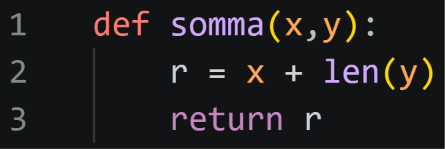
\includegraphics[width=.5\linewidth]{img/f_errata.png}
        \end{figure}
    \end{alertblock}
    \begin{alertblock}{DESCRIZIONE DELLA FUNZIONE}
        \begin{figure}
            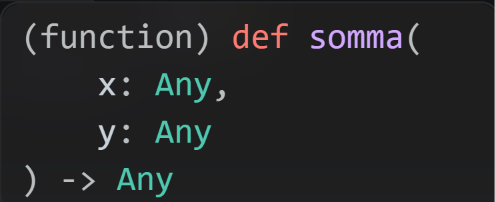
\includegraphics[width=.5\linewidth]{img/f_errata_desc.png}
        \end{figure}
    \end{alertblock}
\end{frame}

\begin{frame}{PARAMETRI DELLE FUNZIONI}
    \begin{alertblock}{COSA RESTITUISCE LA FUNZIONE SOMMA?}
        \begin{figure}
            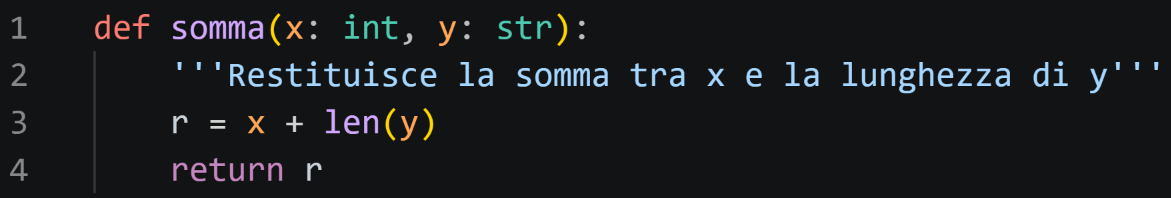
\includegraphics[width=\linewidth]{img/f_corretta.png}
        \end{figure}
    \end{alertblock}
    \begin{alertblock}{DESCRIZIONE DELLA FUNZIONE}
        \begin{figure}
            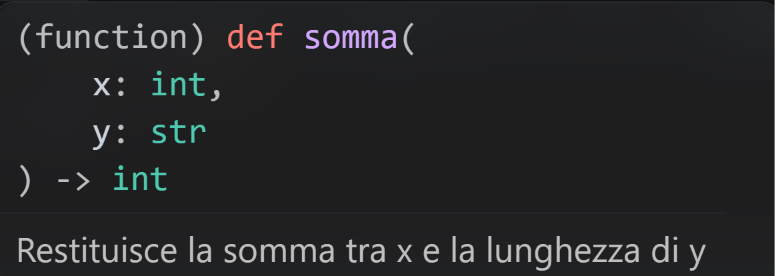
\includegraphics[width=.7\linewidth]{img/f_corretta_desc.png}
        \end{figure}
    \end{alertblock}
\end{frame}

\section{EI IA, RIASSUMI!}

\begin{frame}[fragile]{STRUTTURA DI UN PROGRAMMA}
    \begin{alertblock}{STRUTTURA}
        \begin{minipage}{0.98\linewidth}
\begin{lstlisting}[language=Python]
 import math
 
 # VARIABILI GLOBALI
 X = float(input("Inserisci il primo numero: "))
 Y = float(input("Inserisci il secondo numero: "))
 
 # FUNZIONI
 def somma_intera(num1: float, num2: float):
     '''Dati due numeri ne restituisce la somma intera'''
     return math.floor(num1 + num2)
 
 r = somma_intera(X,Y)
 
 print(f"La somma intera tra i due numeri è: {r}")
\end{lstlisting}
        \end{minipage}
    \end{alertblock}
\end{frame}

\end{document}